\documentclass[border=4pt]{standalone}

\usepackage{tikz}

\definecolor{otblue}{HTML}{0072B2}
\definecolor{otorange}{HTML}{E69F00}
\definecolor{otteal}{HTML}{009E73}
\definecolor{otpurple}{HTML}{CC79A7}
\definecolor{otgray}{HTML}{5A5A5A}

\begin{document}
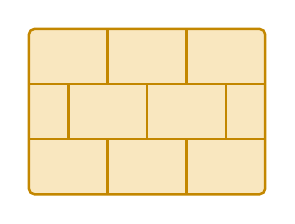
\begin{tikzpicture}[line width=0.9pt]
  \begin{scope}
    \clip[rounded corners=2pt] (0,0) rectangle (3,2.1);
    \fill[otorange!25] (0,0) rectangle (3,2.1);
    \foreach \y in {0.7,1.4}{\draw[otorange!85!black] (0,\y) -- (3,\y);}
    \foreach \x in {1,2}{\draw[otorange!85!black] (\x,0) -- (\x,0.7); \draw[otorange!85!black] (\x,1.4) -- (\x,2.1);}
    \foreach \x in {0.5,1.5,2.5}{\draw[otorange!85!black] (\x,0.7) -- (\x,1.4);}
  \end{scope}
  \draw[otorange!85!black, rounded corners=2pt] (0,0) rectangle (3,2.1);
\end{tikzpicture}
\end{document}
